\documentclass[../thesis.tex]{subfiles}
\begin{document}
\chapter{Technologies and tools}\label{cap:technologies-and-tools}

\section{Tensorflow}
Tensorflow is an open-source Python library to build \acrshort{ML} models. Google started its development in 2015 and today is one of the most used Python libraries to perform \acrshort{ML} tasks. It offers a huge number of layers, activation functions, and tools to build simple and complex neural network architectures.

\subsection{Tensorflow lite}
Tensorflow lite is a component of Tensorflow that allows to convert a Tensorflow model into a compressed flat buffer and then deploy it into any device (e.g.\ mobile devices or embedded device). With the goal of deploying the hand gesture recognizer to a Nvidia Jetson, the use of this tool is natural.

\subsection{Keras}
Keras takes advantages of Tensorflow to give to the user a powerful API to design and develop Deep Neural Networks. With a few lines of code is possible to implement complex neural networks that exploit the latest researches in the field of \gls{ML}.

\section{MediaPipe}\label{sec:mediapipe}
MediaPipe is an open-source, real-time, and on-device tool that can track multiple parts of the body. In particular, I am interested in hand tracking. MediaPipe suits very well for this purpose because it offers a pre-trained \acrshort{ML} model to recognize and track twenty-one landmarks on each hand (figure~\ref{fig:landmarksMediapipe}). In particular, it uses a pipeline composed of two \acrshort{ML} models:
\begin{enumerate}
    \item A palm detector that works on a full image locates the palm and identifies the bounding box around it;
    \item A hand landmark model that works on the cropped image of the palm and returns the hand landmarks considering the depth also. 
\end{enumerate}
\begin{figure}[H]
    \centering
    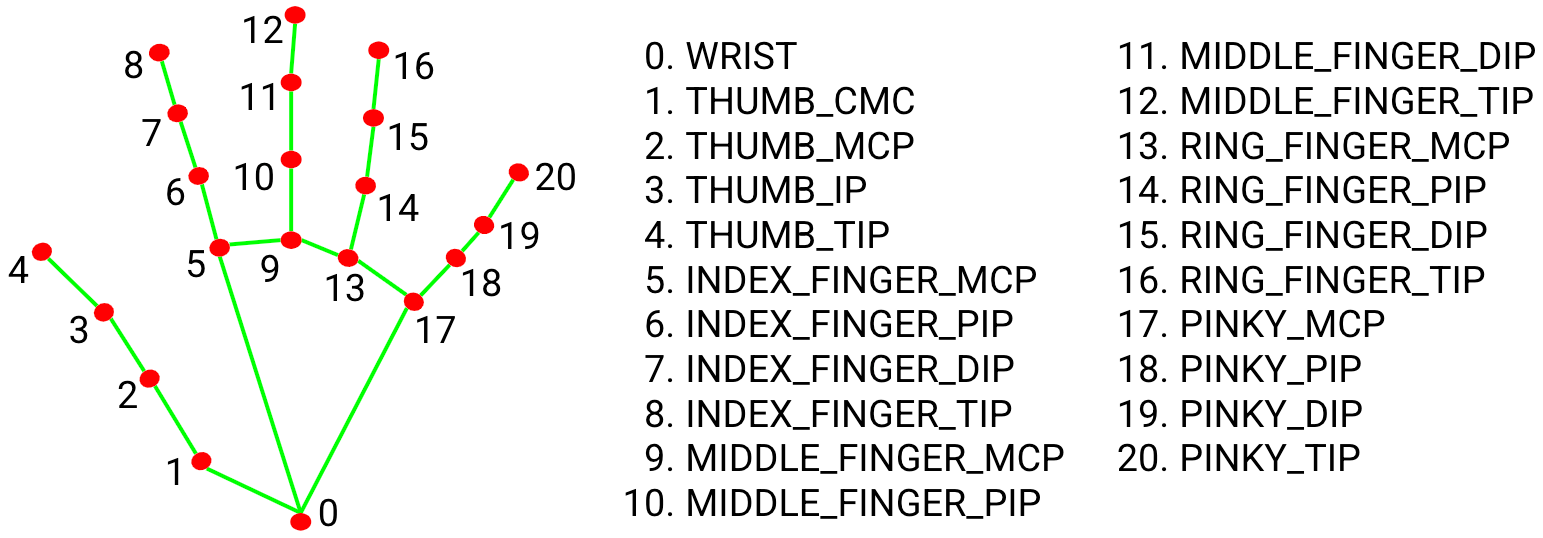
\includegraphics[width=\columnwidth]{mediapipeHandLandmarks.png}
    \caption{Landmarks on a hand recognized by MediaPipe~\cite{site:mediapipe}}
    \label{fig:landmarksMediapipe}
\end{figure}
The precision of this tool is about $96\%$~\cite{article:mediapipe} so, it is a good starting point for the hand gesture recognition task. It is possible to get the position of the landmarks and give them in input at a Deep Neural Network trained on the gestures of our interest.\\
What MediaPipe returns is the list of coordinates relatives at the 2.5D position of hand's landmarks. These coordinates can be saved and used to train a deep neural network instead images, reducing the size of the dataset.\\
It is interesting to point out that MediaPipe is capable to track, in real-time, different parts of a human body, for example, the face and the whole body.~\cite{site:mediapipe}

\section{Robot Operating System}
\acrfull{ROS} is an open-source set of libraries and tools to develop robot applications. The latest \acrshort{LTS} release, and the one used for this project, is \textit{ROS Foxy Fitzroy}. The key points to understand when using \acrshort{ROS} are related to the ``ROS 2 Graph'', and they are:
\begin{itemize}
    \item \textbf{Node}: it is a component of the system responsible for a task. It is an executable, in my case a Python executable but it could also be a C++ executable, and it can communicate with other nodes exchanging messages. A robotic system is composed of multiple nodes;
    \item \textbf{Message}: what nodes use to exchange data. Each message has its own ``type'', and this brings advantages in building an interchangeable system because it is possible to change the components of the system with others that can understand the same messages. Messages, in this case, can be seen as the interfaces for programming languages. There are three ways for nodes to exchange messages:
        \begin{itemize}
            \item \textbf{Topic};
            \item \textbf{Service};
            \item \textbf{Action}.
        \end{itemize}
\end{itemize}
\subsection{Exchange messages}
\subsubsection{Topic}
It is an implementation of the publisher/subscriber pattern. A node can publish messages with a topic, and every other node that is listening to that topic will read that message. This is an asynchronous way to exchange messages because the sender will not know if the message has been read for that this is the best way to broadcast a message without saturating the network.
\begin{figure}[H]
    \centering
    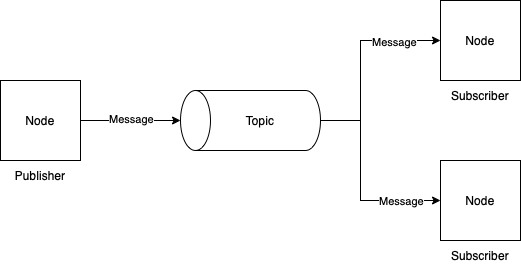
\includegraphics[width=0.7\columnwidth]{topicExample.png}
    \caption{Example of message exchange between three nodes using a topic.}
    \label{fig:exampleTopicExchangeMessage}
\end{figure}

\subsubsection{Service}
It is based on a call-response model. In this case, a node requests some data to another node through a request message. The latter replies with a response message. This is a synchronous way to exchange messages. The node that needs the data waits for the response. There can be many nodes that use the same service to request some data from another node. This is a bit like what happens in a client-server architecture but it should not be used for long running process.
\begin{figure}[H]
    \centering
    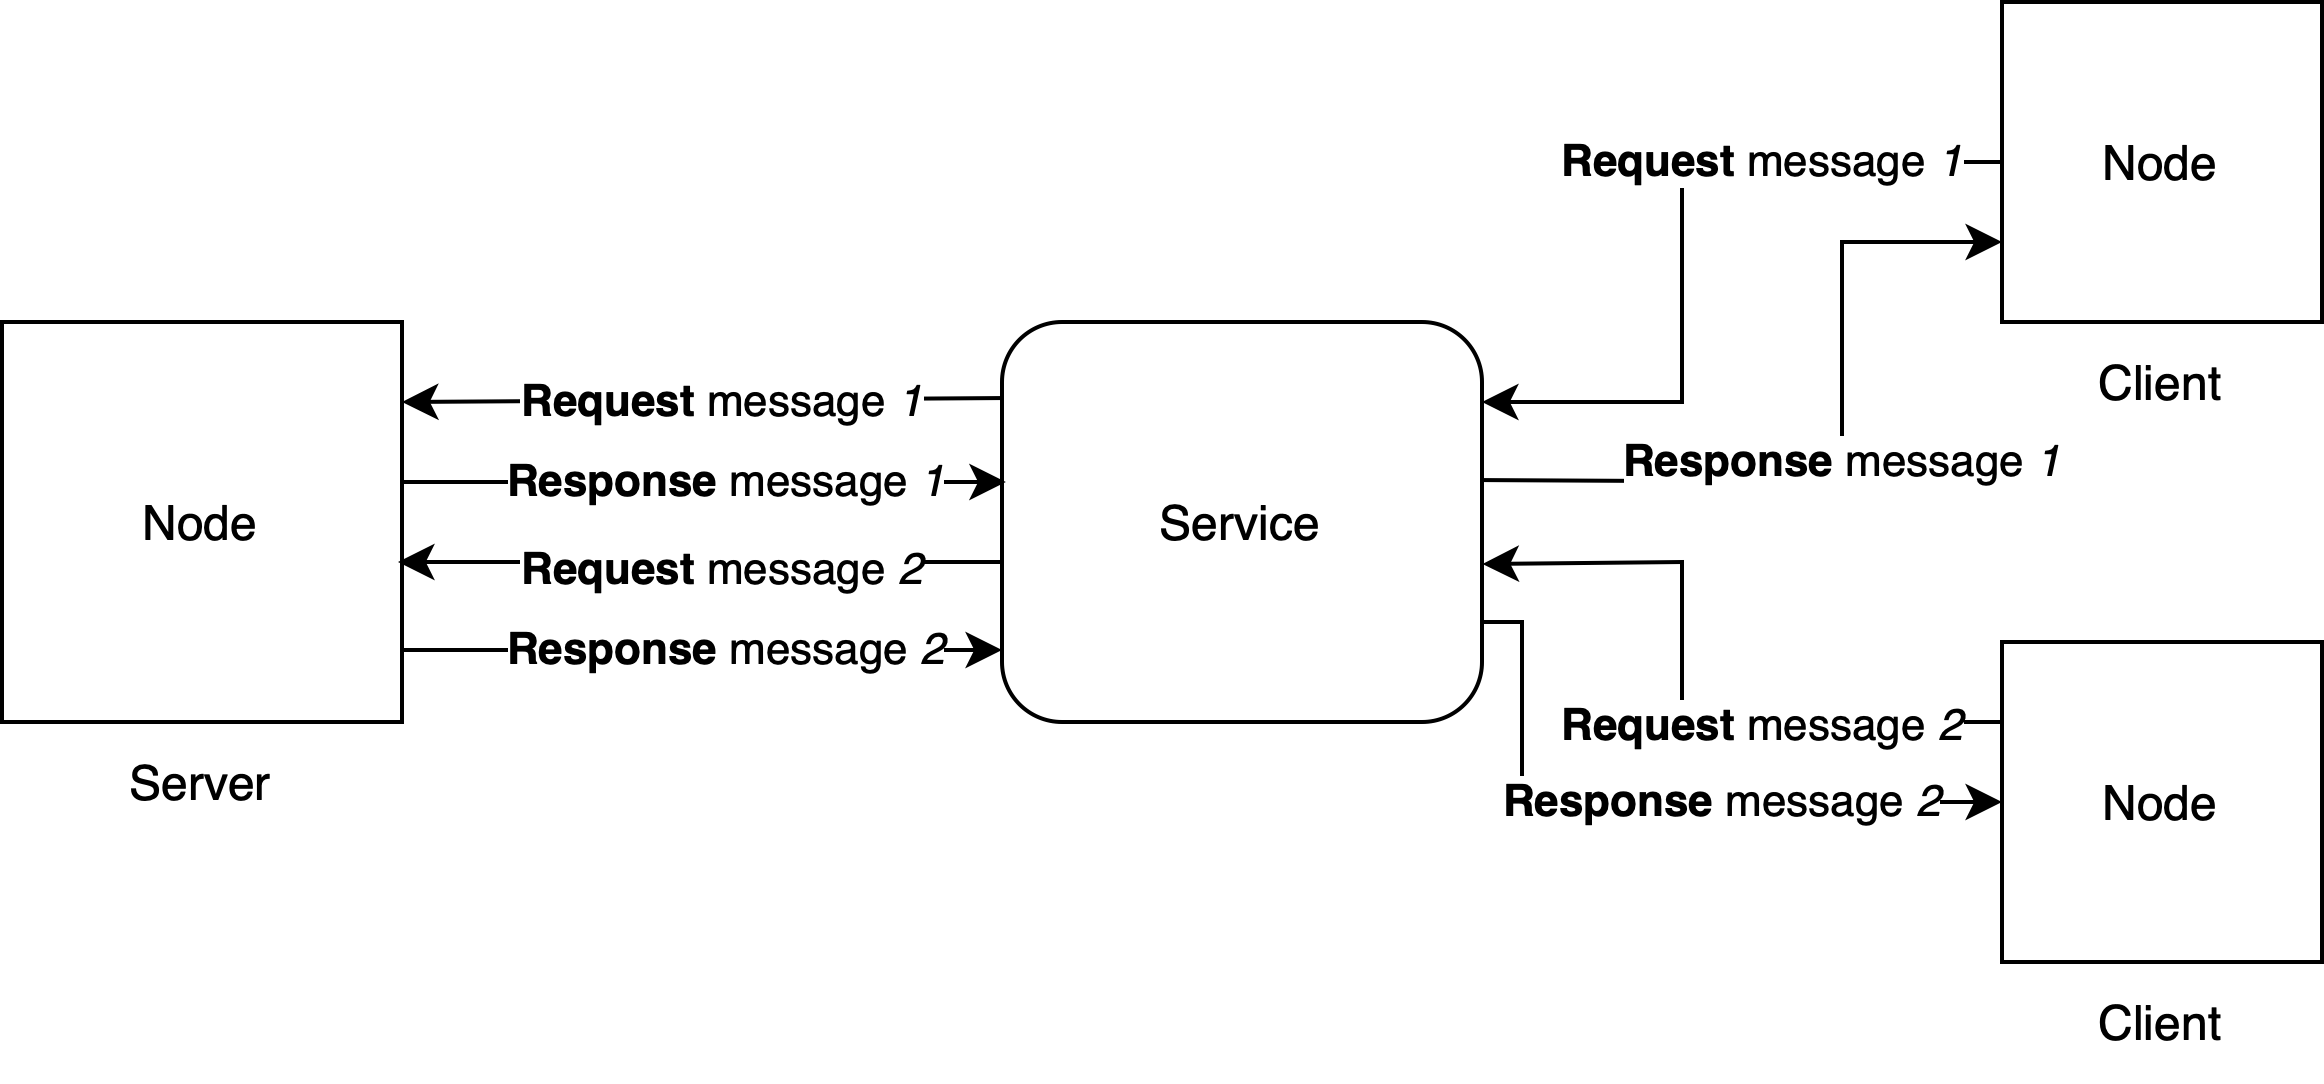
\includegraphics[width=0.8\columnwidth]{serviceExample.png}
    \caption{Example of messages exchange between three nodes using a service.}
    \label{fig:exampleServiceExchangeMessage}
\end{figure}

\subsubsection{Action}
It uses both topics and services. The functionality is similar to service with the addition of a constant stream of updates from the ``server'' through a topic at which the ``client'' subscribes. The sequence of actions is the following:
    \begin{enumerate}
        \item A node (i.e.\ the client) sends a message (the request for a goal) through a service to another node (i.e.\ the server). The latter replies with one message through the service. For example, it can reply with an acknowledgment or a message saying it starts working on a task;
        \item The server keeps the client updated with the progress of the task through a topic;
        \item The client sends a request through another service to the server. When the task finishes, the server will reply to the client.
    \end{enumerate}
\begin{figure}[H]
    \centering
    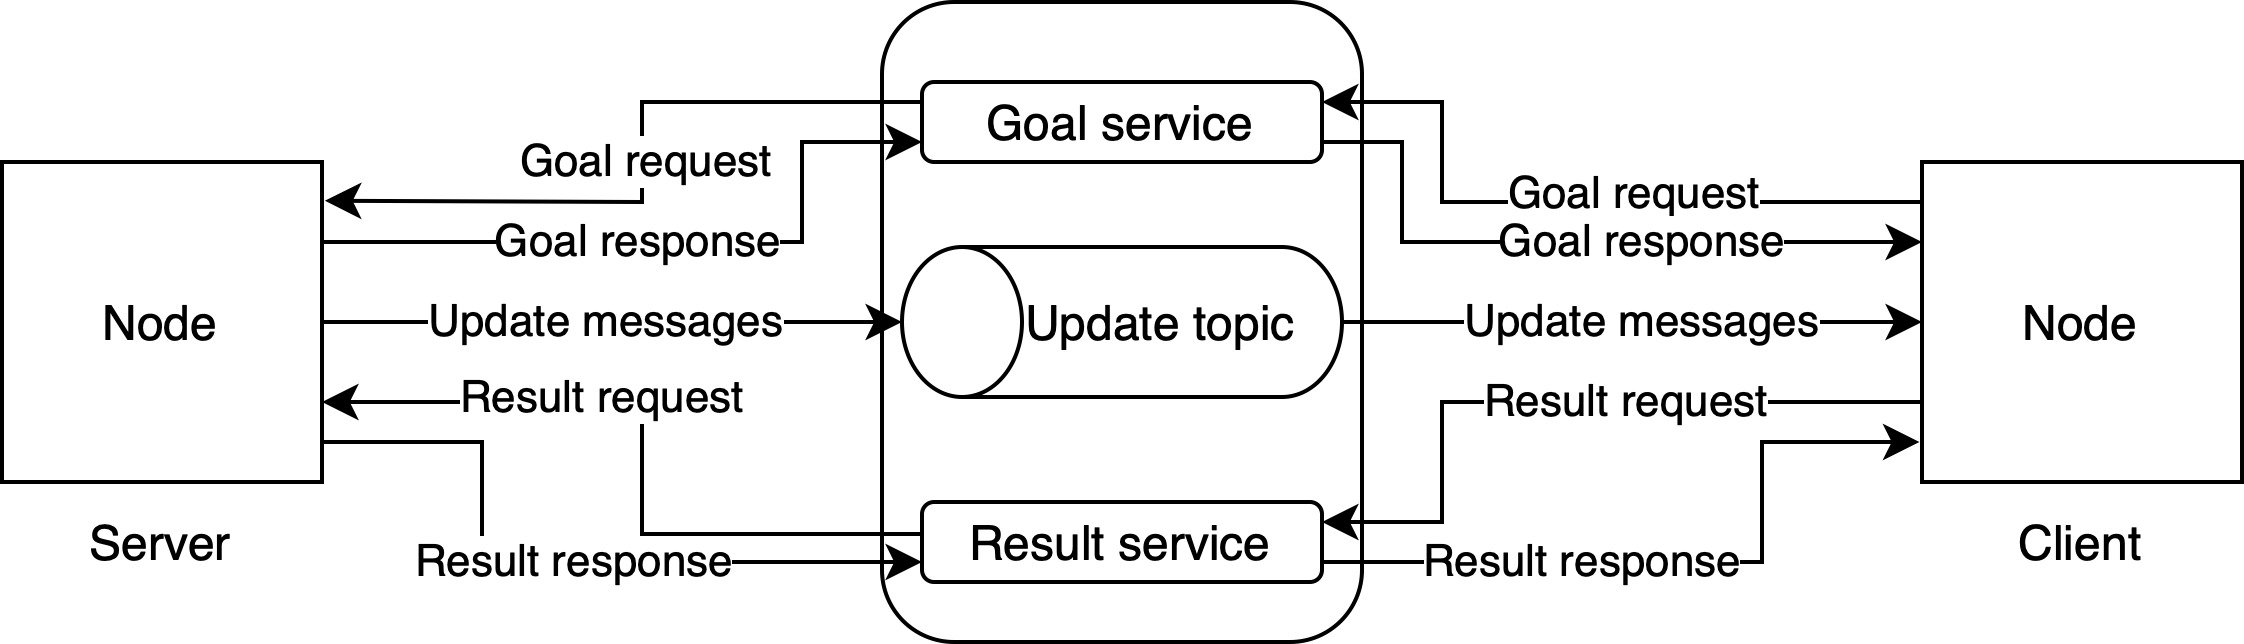
\includegraphics[width=1\columnwidth]{actionExample.png}
    \caption{Example of messages exchange between two nodes using an action.}
    \label{fig:exampleActionExchangeMessage}
\end{figure}

\subsection{Communication between nodes over the network}
\gls{ROS} uses \glsfirst{DDS} as an end-to-end middleware to exchange messages:  This difference is one of the mains between \gls{ROS} version 1 and \gls{ROS} version 2. \gls{DDS} was chosen by \gls{ROS} maintainer for its reliability and flexibility in mission-critical systems, such as:
\begin{itemize}
    \item battleships;
    \item large utility installations;
    \item financial systems;
    \item space systems;
    \item flight systems;
    \item train switchboard systems.
\end{itemize}
The implementation of \gls{DDS} is hidden from the user, who uses the three methods described above with the \gls{ROS} API to exchange messages. More information can be found on the article written by \citeauthor{site:ros_dds}~\cite{site:ros_dds}.

\subsection{Navigation}
``Nav 2'' is the navigation system provided by \gls{ROS}. A developer can chose to use their own navigation system but the one developed by ~\citeauthor{paper:navigation2} is widely tested and supported~\cite{paper:navigation2}. 

\section{Gazebo simulator}
Gazebo is an open-source simulator that allows simulating environments where robots are involved. Gazebo offers the ability to accurately and efficiently simulate populations of robots in complex indoor and outdoor environments. Moreover, there is the possibility to use different robot models using \glsfirst{SDF} file and to import Collada file into the simulated world. Gazebo is also expandable with plugins. One of those allows using \acrshort{ROS} to communicate with the robots inside the simulation. I used the Gazebo simulator to perform some tests before deploying the software in a real environment. 
\end{document}
